% !TeX spellcheck = en_US
% !TEX root = ../thesis-example.tex
%
\section{Chroma Key}
\label{sec:chromakey}

Beginning from a real-
world camera, the video signal travels through the 
Inogeni 4KUSB3 converter and is accessible with the systems API for webcams. 
(See figure \ref{fig:system-components})

\begin{figure}[htb]
	\centering
	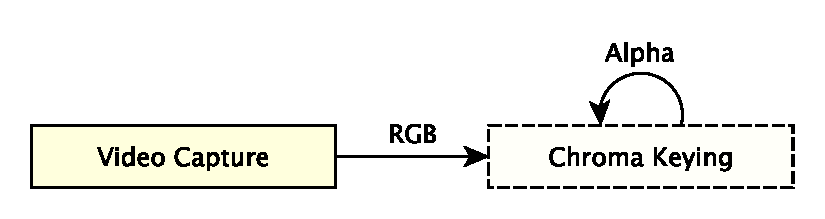
\includegraphics[width=.7\textwidth]{_raw_resources/pipeline_steps/4_1_chroma.pdf}
	\caption{Initial step upon receiving the camera image}
	\label{fig:steps:chroma}
\end{figure}

The initial step is to remove the green (or blue) background from the image, 
which should be live footage of a green (or blue) box. Other literature usually 
refers to it as "pulling a video matte" or "chroma keying." For a reference 
green, there has to be a color picked manually in the material editor of Unity 
- this was made by a checkbox to show raw output from the camera (eg. fig. 
\ref{fig:chroma:editor}). Then an average green from the background box can be 
picked. This is an important setup step, since lightning situations can vary 
greatly and minor differences in light setups can have a great effect on the 
outcome of visible green background captured by the camera, thus making a 
recalibration necessary.

\begin{figure}[htb]
	\centering
	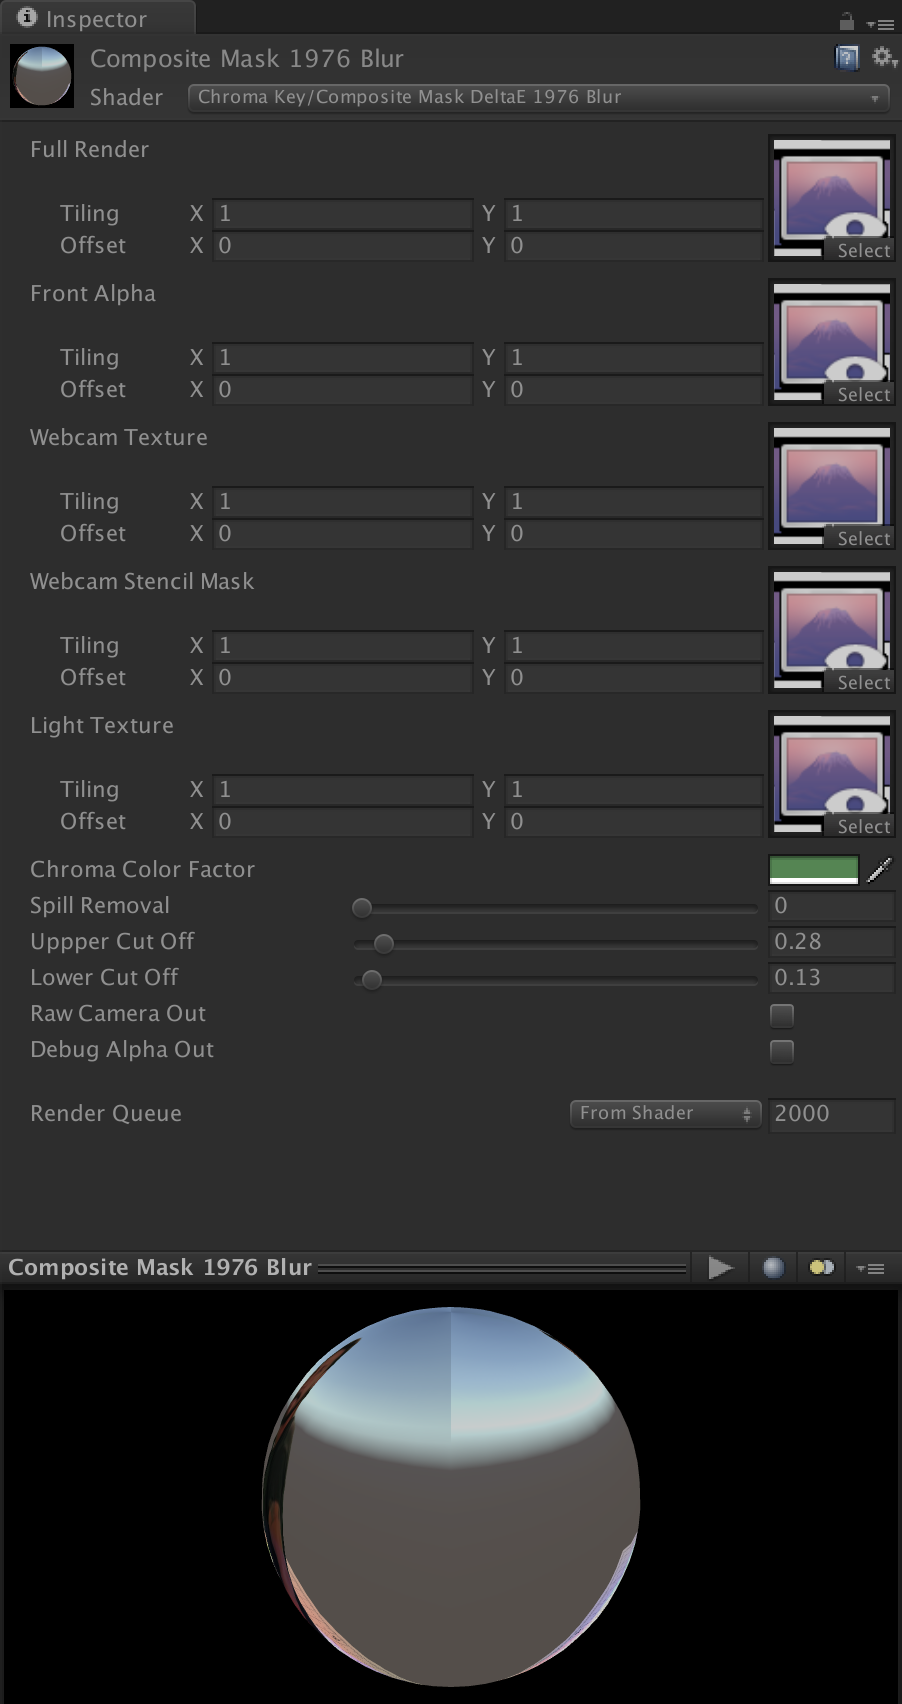
\includegraphics[width=.45\textwidth]{gfx/distances/material-editor.png}
	\caption{Material Editor inside Unity}
	\label{fig:chroma:editor}
\end{figure}

An extreme example case is used for comparing different chroma keying variants, 
which shows high motion blur due to a low shutter speed of the capturing 
camera and fast movement of the depicted actor:

\begin{figure}[htb]
	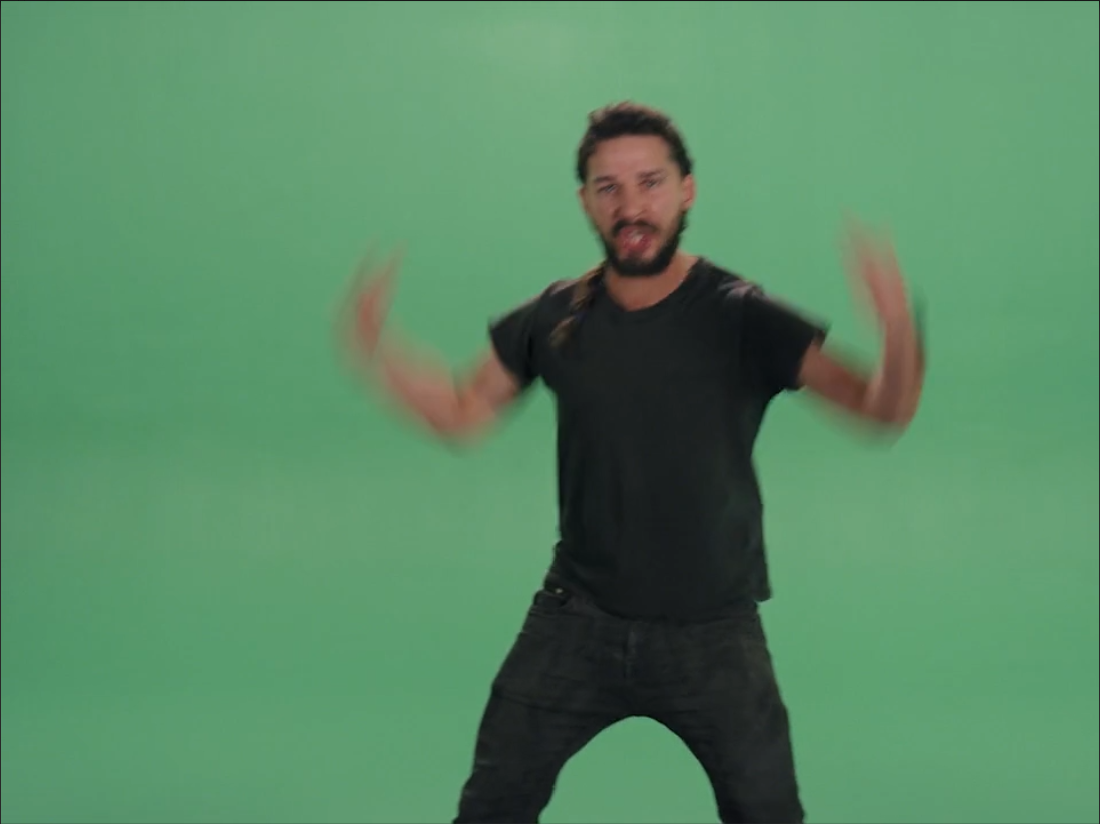
\includegraphics[width=\textwidth]{_raw_resources/Comparison_Example.png}
	\caption{Comparison Image \cite{vimeo:shia:2015} - sRGB Output}
	\label{fig:chroma:color}
\end{figure}

\subsection{Initial Assumption}

Each RGB color can be represented as a discrete 3-Vector of (red, green and 
blue)  values in range of $[0, 1]$\footnote{Software RGBA color representations 
usually take 8bit per color channel and map between $[0, 255]$ - graphic 
computing usually maps between $[0, 1]$}. An interpolation between two colors 
can be summarized as a matting equation as follows, where a foreground image 
$C_F$ and a background image $C_B$ - $\alpha_B$ is assumed to be $1$:

\eq{eq:chroma:assumption:alpha:1}{
	I_{x, y} = \alpha_{x, y} C_{F_{x, y}} + (1 - \alpha_{x, y}) C_{B_{x, y}}
}

This matting equation has to be generalized for a later step, where 
$\protect\alpha$ is a value between [0, 1] on fore- and background, yielding a 
total Alpha of $\alpha_T$ as following:

\eq{eq:chroma:assumption:alpha:weak}{
	\alpha_T = \alpha_B * (1 - \alpha_F) \\
}

thus:

\eq{eq:chroma:assumption:alpha:cont}{
	I_{x, y} = (1 - \alpha_T) F_{x, y} + \alpha_T B{x, y}
}

This equation can take $\alpha_T < 1$ into account, which is needed later when 
fore- and background of the virtual environment are merged with a layer in 
between that results from the real world capture.

\subsection{Euclidean RGB Distance}
Assuming a source pixel color $C_S$ and a reference color $C_R$ we can 
calculate the euclidean distance between these two color vectors:
\eq{eq:euclidianrgb}{
	\alpha = \sqrt{(C_RR - C_SR)^2 + (C_RG - C_SG)^2 + (C_RB - C_SB)^2}
}

\begin{figure}[htb]
	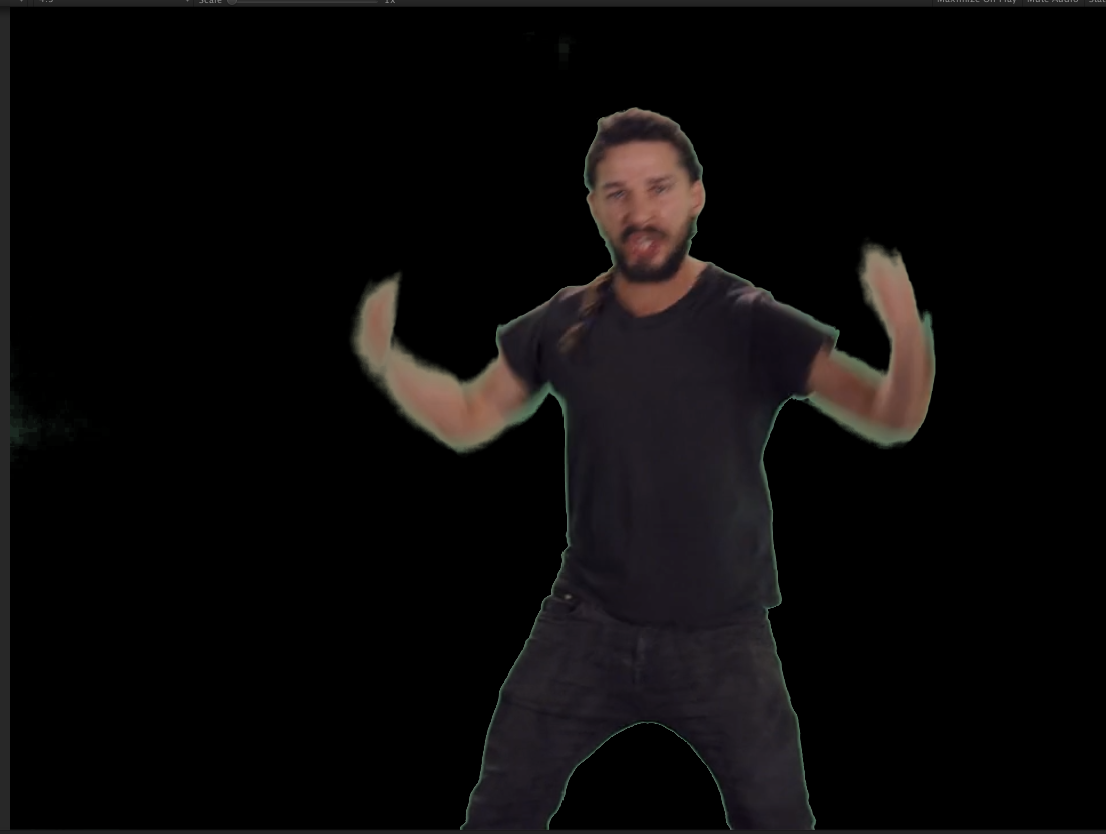
\includegraphics[width=\textwidth]{_raw_resources/Comparison_RGB_color.png}
	\caption{Chroma Keying by using euclidean RGB distance}
	\label{fig:chroma:euclidean:rgb}
\end{figure}

This is computationally very low cost and works well enough to detect a 
difference between two distinct colors. It fails to accommodate for coloring 
that is perceived as different, but tinted by the reference colors. Since the 
green screen material will never achieve 0\% reflectivity, some color will 
spill onto the filmed actor and will therefore generate unwanted chroma-keying 
artifacts, most noticeable on semi-glossy reflection of skin or color tints on 
white clothing.

\subsection{Euclidean YCgCo Distance}

YCgCo gets its name for Luminance (Y), chrominance green (Cg) and chrominance 
orange (Co) and helps decorrelating color spaces by splitting color-lightness 
from color chrominances, thus splicing the color model into brightness and 
color appearance. Since it is a fast, lossless color transformation it 
is used in example for H.264 video encoding and other image compression 
techniques. The two chrominance channels are then split into green to magenta 
and orange to blue color channels and allow for a more accurate distance 
calculation between two colors.

\begin{figure}[htb]
	\includegraphics[width=\textwidth]{_raw_resources/Comparison_YCgCo_color.png}
	\caption{Chroma Keying by using euclidean YCgCo distance}
	\label{fig:chroma:euclidean:ycgco}
\end{figure}

Transforming any RGB color to YCgCo can be done with a single matrix  
multiplication, which is - again - a very low-cost computation on a GPU:

\eq{eq:ycgco:transformation}{
	\begin{bmatrix}
		Y \\
		Cg \\
		Co \\
	\end{bmatrix}
	=
	\begin{bmatrix}
		 \frac{1}{4} && \frac{1}{2} &&  \frac{1}{4} \\
		-\frac{1}{4} && \frac{1}{2} && -\frac{1}{4} \\
		 \frac{1}{2} && 0           && -\frac{1}{2}
	\end{bmatrix}
	*
	\begin{bmatrix}
		R \\
		G \\
		B 
	\end{bmatrix}
}

Given two colors, one from the video source $C_S$ and a reference color $C_R$ 
it is now possible to calculate the euclidean distance on the two chrominance 
channels:

\eq{eq:ycgco:euclidean}{
	\alpha = \sqrt{(C_RCg - C_SCg)^2 + (C_RCo - C_SCo)^2}
}

Due to the increased decorrelation, the result is more accurate and shows less 
artifacts on target pixels, allowing for better matte pulling, less 
green edges and a more continuous, smooth image of an actor.

\subsection{Euclidean Lab Difference}
The International Color Consortium (ICC) defined 1976 \textit{Lab $\Delta$E} as 
a standard model of calculating color differences inside the \textit{Lab} color 
vector volume. The final distance calculation is a linear euclidean scalar as 
with all other models, but accommodates for perceived color differences. It is 
a more expensive computation and needs code branches, which will evaluate all 
branches first by the GPU before using either code path.

A reference white has to be used to convert RGB to the Lab color model to 
accommodate for different RGB color spaces\footnote{which are usually only 
different on stored image material like photos or video}. Luckily the given 
webcam signal defaults to sRGB D65 and does not need a configurable reference 
matrix based on a given color model to handle different RGB color standards.

sRGB conversion needs to be converted to linear RGB while respecting light 
energy per color channel, rather than relative, perceived color brightness: 

\eq{chroma:inversecompanding}{
	v \in \{r, g, b\} \land V \in \{R, G, B\}
}

where: 

\eq{chroma:inverseRGBcompanding}{
	v = \\
	\begin{cases}
		V / 12.92                   & \quad \text{if } V \leq 0.0405 \\
		((V + 0.055) / 1.055)^{2.4} & \quad \text{otherwise}
	\end{cases}
}

from there an linear RGB color can be converted to XYZ by the following 
equation:

\eq{chroma:conversioncalc}{
	\begin{bmatrix}
		X\\
		Y\\
		Z\\
	\end{bmatrix}
		=
	\begin{bmatrix}
		M
	\end{bmatrix}
	\begin{bmatrix}
		R\\
		G\\
		B\\
	\end{bmatrix}
}

where:

\eq{chroma:rgbmatrix}{
	\begin{bmatrix}
		M
	\end{bmatrix}
		=
	\begin{bmatrix}
		R X_r && G X_g && B X_b \\
		R Y_r && G Y_g && B Y_b \\
		R Z_r && G Z_g && B Z_b
	\end{bmatrix}
}


\eq{chroma:xyzmatrix}{
		\begin{bmatrix}
		X\\
		Y\\
		Z\\
	\end{bmatrix}
	\begin{bmatrix}
		M
	\end{bmatrix}
	=
	\begin{pmatrix}
		X_r / Y_r && X_g / Y_g && X_b / Y_g \\
		1 && 1 && 1 \\
		\frac{1-X_r-Y_r}{Y_r} && \frac{1-X_g-Y_g}{Y_g} && \frac{1-X_b-Y_b}{Y_b}
	\end{pmatrix}
}

The needed $\begin{bmatrix}M\end{bmatrix}$ for RGB D65 is defined as:

\eq{chroma:sRGBD65}{
	\begin{bmatrix}
		0.4124564 && 0.3575761 && 0.1804375 \\
		0.2126729 && 0.7151522 && 0.0721750 \\
		0.0193339 && 0.1191920 && 0.9503041 \\
	\end{bmatrix}
}

Based on a reference white $U_r \in \{X_r, Y_r, Z_r\}$:

\eq{chroma:xyz2lab:defines}{
	U \in \{X, Y, Z\} \land W \in \{L, a, b\}
}

\eq{chroma:xyz2lab:epsilon}{
	\epsilon = 0.008856 \land \kappa = 903.3
}

where:

\eq{chroma:xyz2lab:ref}{
	w_r = \frac{U}{U_r}
}

\eq{chroma:xyz2lab:channel}{
	f(w) = \\
	\begin{cases}
		\sqrt[3]{w_r}      & \quad \text{if } U > \epsilon \\
		\frac{\kappa w_r + 16}{116} & \quad \text{otherwise}
	\end{cases}
}


\eq{chroma:xyz2lab:conversion}{
	\begin{bmatrix}
		L \\
		a \\
		b \\
	\end{bmatrix}
	=
	\begin{bmatrix}
		116 f_y - 16 \\
		500 (f_x - f_y) \\
		200 (f_y - f_z)
	\end{bmatrix}
}

With this conversion from sRGB to linear RGB to XYZ to Lab we can now calculate 
the euclidian linear distance between two colors $C_S$ and $C_R$, which already 
have been converted to Lab:

\eq{chroma:cie76:distance}{
	\Delta E = \sqrt{(C_R L - C_S L)^2 + (C_R a - C_S a)^2 + (C_R b - C_S b)^2}
}

The resulting values are rated by their perceptive difference (after Mkrzycki 
et. al. \cite{mokrzycki:2012}):

\begin{tabular}[htb]{l | l}
	0.0 \dots 0.5 & the difference is unnoticeable \\
	0.5 \dots 1.0 & the difference is only noticed by an experienced observer \\
	1.0 \dots 2.0 & the difference is also noticed by an unexperienced observer 
	\\
	2.0 \dots 4.0 & the difference is clearly noticeable \\
	4.0 \dots 5.0 & fundamental color difference  \\
	> 5.0 		  & gives the impression that these are two different 
	colors
\end{tabular}

Now it's possible to map alpha values for each pixel based on $\Delta$E 
distances between $m, n$ by clamping and biasing $\Delta$E with a proposed 
"smooth step" algorithm:

\eq{chroma:cie76:clamp}{
	f({\Delta E}) = x = \frac{\Delta E - n}{m - n}
}

\eq{chroma:cie76:min/max}{
	g(f({\Delta E})) = y =
	\begin{cases}
		n        & \quad \text{if } x \leq n \\
		x        & \quad \text{if } n \leq x \leq m \\
		m        & \quad \text{if } m \leq x
	\end{cases}
}

\eq{chroma:cie76:mapping}{
	\alpha(I_{x, y}) = 3 y ^2 - 2 y ^3
}

With that we receive a more natural matte with nearly no green edges, 
continuous actor imagery and smooth alpha transition between actor and green 
screen. Motion blur is hard to account for and is even with professional video 
matting hardware, extensive post production or intrinsic frame matting 
algorithms hard to remove without rough image results.

\begin{figure}[htb]
	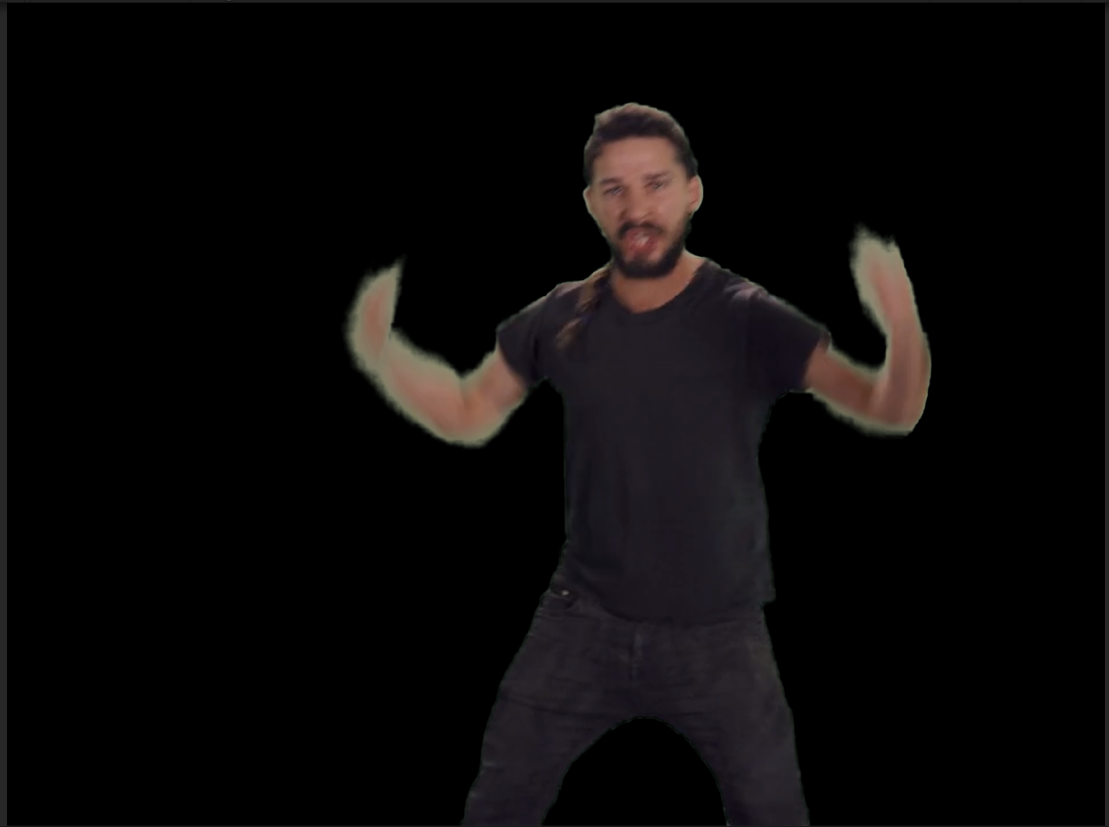
\includegraphics[width=\textwidth]{_raw_resources/Comparison_DeltaE_color.png}
	\caption{Chroma Keying by using $\protect\Delta $E distance}
	\label{fig:chroma:deltae}
\end{figure}

\subsection{Comparison between computational models}

To chose the best variant, balancing runtime and efficiency, there has to be a 
comparison between the presented methods. Again, the previous image will be 
used, since it has complicated color mixing between background and actor. First 
we pick scan line of the image, in this case the 301st row from top, and 
calculate the color distance from each pixel to a reference color $[R, G, B] = 
[0.341, 0.588, 0.42]$.

As seen in figure \ref{fig:chroma:image_comparison}d, CIEDE76s performance is 
significantly better in separating colors and has a broader margin between 
green background and other foreground. This can be observed in figure 
\ref{fig:chroma:image_comparison}, where the scan line is set as background and 
the values are normalized again:

\begin{figure}[htbp]
	\caption{Comparison between different color distance methods}
	\label{fig:chroma:image_comparison}
	\begin{subfigure}[t]{.65\textwidth}
		\centering
		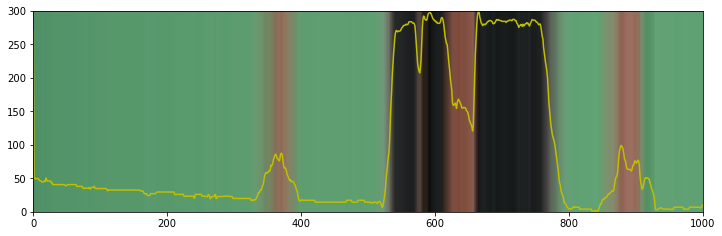
\includegraphics[width=\textwidth]{gfx/distances/color-rgb.png}
		\caption{RGB color distance} 
	\end{subfigure}
	\begin{subfigure}[t]{.3\textwidth}
		\centering
		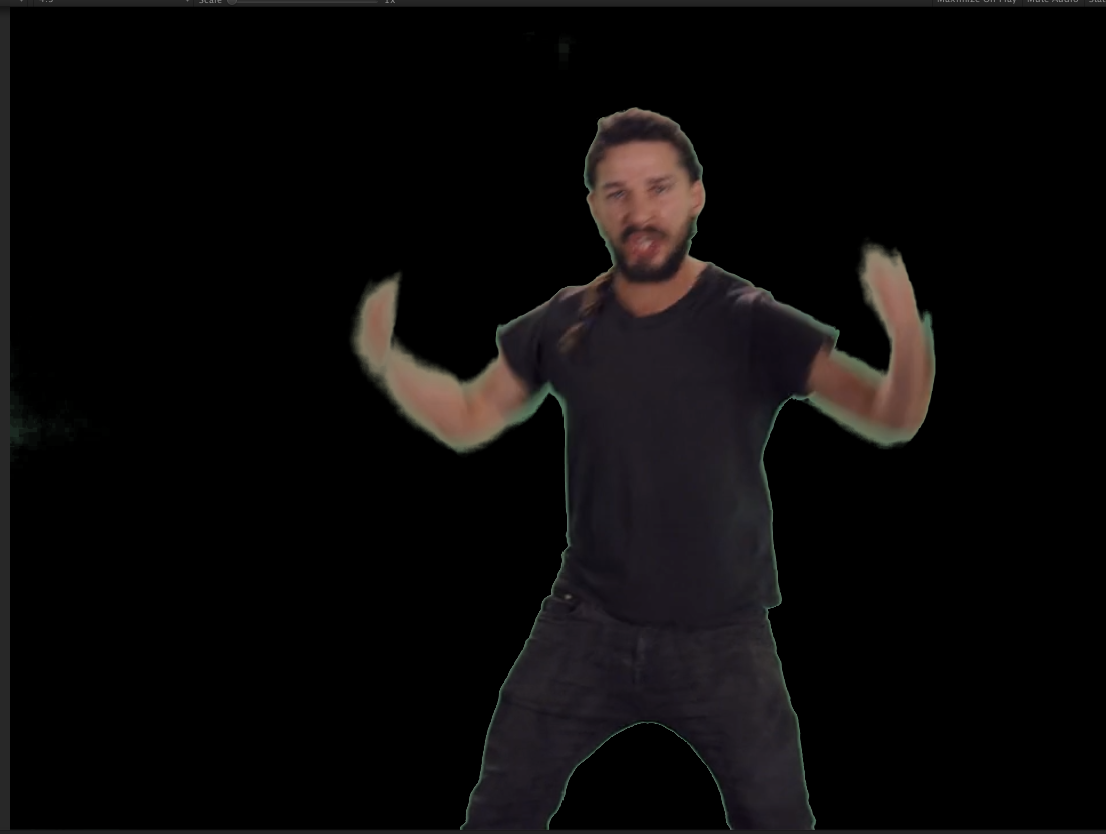
\includegraphics[width=\textwidth]{_raw_resources/Comparison_RGB_color.png}
	\end{subfigure}
	\begin{subfigure}[t]{.65\textwidth}
		\centering
		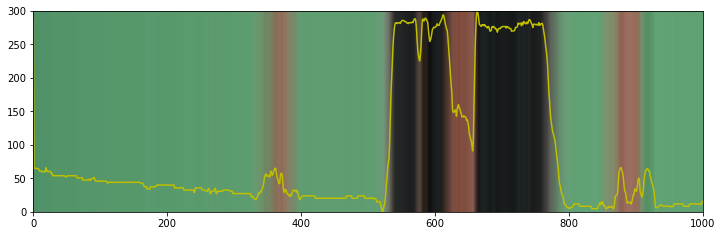
\includegraphics[width=\textwidth]{gfx/distances/color-ycgco.png}
		\caption{YCgCo color distance}
	\end{subfigure}
	\begin{subfigure}[t]{.3\textwidth}
		\centering
		\includegraphics[width=\textwidth]{_raw_resources/Comparison_YCgCo_color.png}
	\end{subfigure}
	\begin{subfigure}[t]{.65\textwidth}
		\centering
		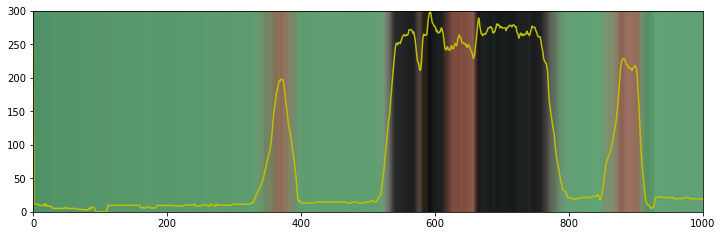
\includegraphics[width=\textwidth]{gfx/distances/color-ciede76.png}
		\caption{CIEDE76 color distance}
	\end{subfigure}
	\begin{subfigure}[t]{.3\textwidth}
		\centering
		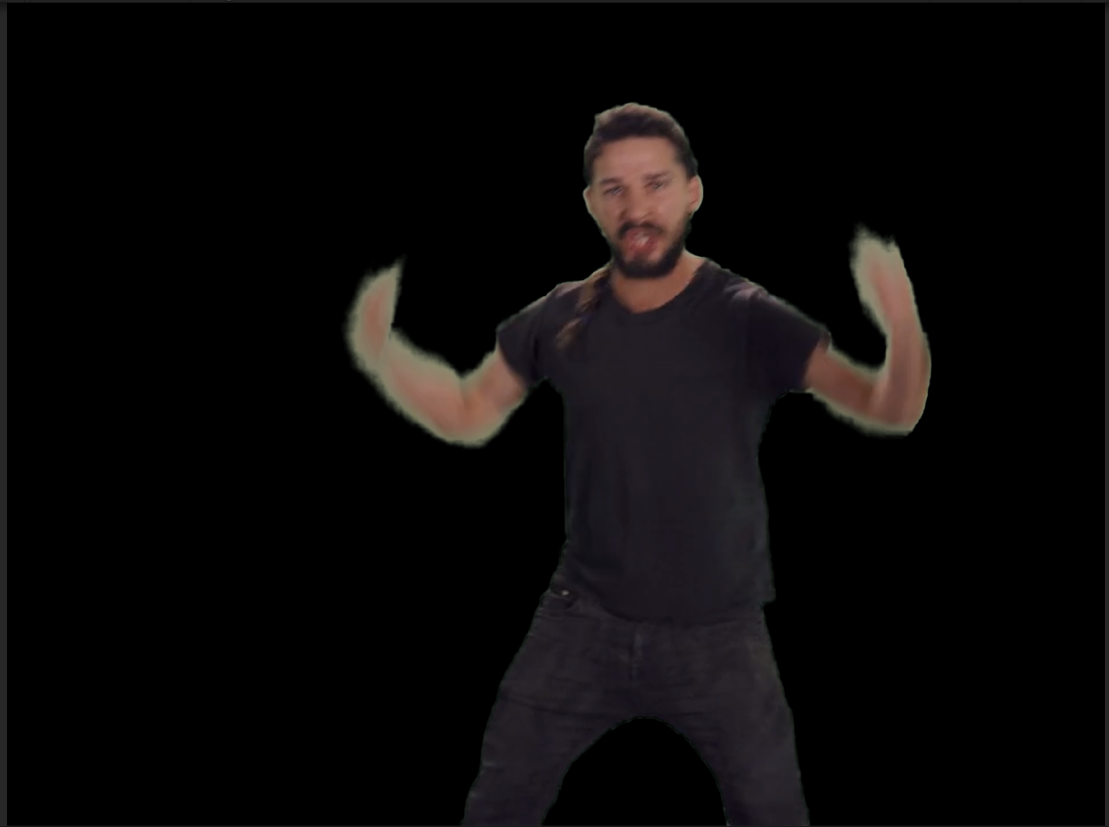
\includegraphics[width=\textwidth]{_raw_resources/Comparison_DeltaE_color.png}
	\end{subfigure}
	\begin{subfigure}[t]{\textwidth}
		\centering
		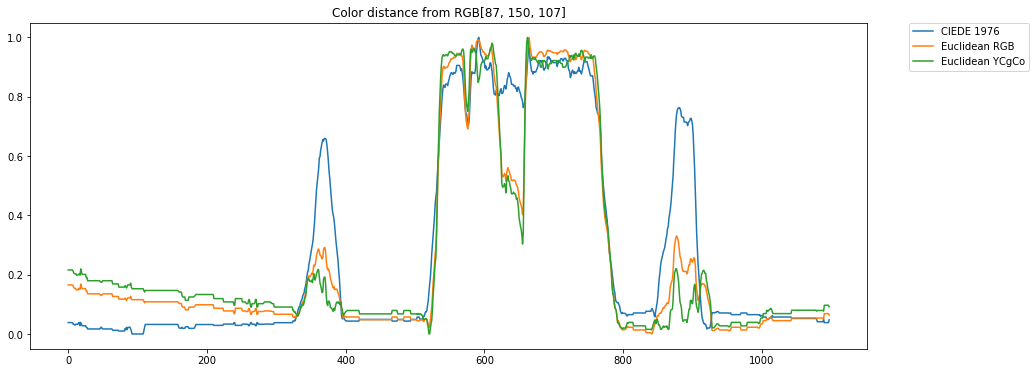
\includegraphics[width=\textwidth]{gfx/distances/dist-comp.png}
		\caption{Normalized graph comparing color difference methods}
	\end{subfigure}
	\begin{subfigure}[t]{\textwidth}
		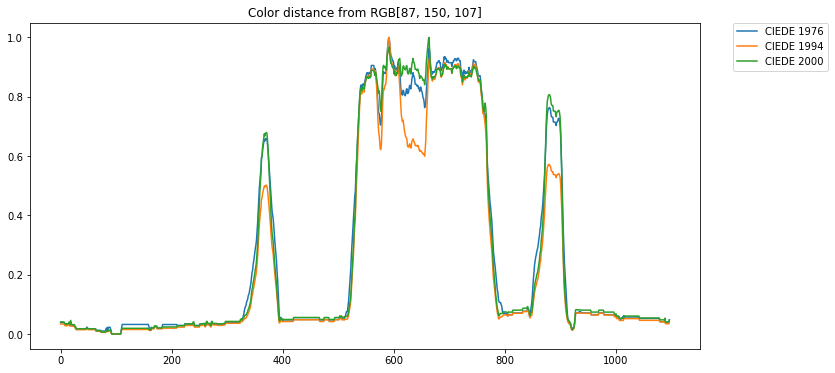
\includegraphics[width=\textwidth]{gfx/distances/ciede-comp.png}
		\caption{Comparison with different CIEDE $\Delta E$ variants}
	\end{subfigure}
\end{figure}
Additionally, CIEDE76 shows less variance on similar colored spaces to the 
target color as well as high color difference peaks on all other pixels. This 
yields an accurate upper and lower limit, in which the green screen can be 
calibrated in.
\newline
Finally, comparing CIEDE76, CIEDE94 and CIEDE2000 reveals, that CIEDE76 
performs well enough while having the lowest performance overhead. The 
similarities between the 1976 and 2000 method are very apparent, while 
CIEDE2000 has a significantly more complex algorithm. (cf.  
\cite{sharma:ciede2000:2005}) Performing the same operation on the same data 
with different CIEDE color distance revisions (fig. 
\ref{fig:chroma:image_comparison}e), that there is little difference between 
CIEDE76 and CIEDE2000.